\section{PHƯƠNG TRÌNH TRẠNG THÁI KHÍ LÍ TƯỞNG}
\subsection{LÝ THUYẾT TRỌNG TÂM}
\subsubsection{Phương trình trạng thái của khí lí tưởng}
\begin{boxdl}
	Phương trình trạng thái của một lượng khí lí tưởng xác định:
	\begin{equation}
		\dfrac{pV}{T}=\text{hằng số}\quad \text{hay}\quad \dfrac{p_1V_1}{T_1}=\dfrac{p_2V_2}{T_2}
	\end{equation}
\end{boxdl}

\subsubsection{Quá trình đẳng tích}
\begin{boxdl}
	Từ phương trình trạng thái, ta rút ra được phương trình liên hệ giữa áp suất và nhiệt độ tuyệt đối khi thể tích khí không đổi:
	\begin{equation}
		\dfrac{p}{T}=\text{hằng số}\quad \text{hay} \quad \dfrac{p_1}{T_1}=\dfrac{p_2}{T_2}
	\end{equation}
\end{boxdl}
Đường biểu diễn sự phụ thuộc của $p$ theo $T$ khi thể tích của khối khí không đổi gọi là \textbf{đường đẳng tích}.
\begin{center}
	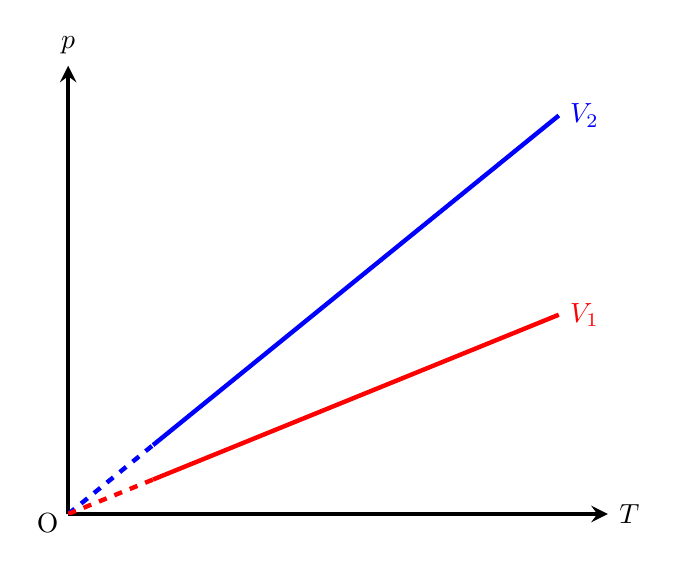
\begin{tikzpicture}  
		\begin{axis}[  ultra thick,
			xmin=0,  
			xmax=1100,  
			xtick=\empty,
			ytick=\empty,
			ymin=0,  
			ymax=900, 
			samples=300,
			xticklabels=\empty,
			yticklabels=\empty,
			axis lines=center, 
			xlabel=$T$, 
			ylabel=$p$, 
			every axis y label/.style={at=(current axis.above origin),anchor=south},  
			every axis x label/.style={at=(current axis.right of origin),anchor=west},  ]
			\addplot [ultra thick, blue, smooth,dashed, domain=0:173] {0.8*x}; 
			\addplot [ultra thick, blue, smooth, domain=173:1000] {0.8*x} node[right]{$V_2$}; 
			\addplot [ultra thick, red, smooth,dashed, domain=0:173] {0.4*x}; 
			\addplot [ultra thick, red, smooth, domain=173:1000] {0.4*x} node[right]{$V_1$};
		\end{axis}  
		\node[label={[below left]90:O}] at (0,0){};
	\end{tikzpicture}
	\captionof{figure}{Các đường đẳng tích của một khối khí lí tưởng ứng với các thể tích $V_1$ và $V_2 \left(V_2<V_1\right)$}
\end{center}
\subsection{VÍ DỤ MINH HOẠ}
\begin{dang}{Sử dụng định luật Boyle và định luật Charles rút ra được phương trình trạng thái của khí lí tưởng}
\end{dang}
\begin{vd}
	Xét một khối khí lí tưởng xác định biến đổi từ trạng thái 1 $\left(p_1, V_1, T_1\right)$ sang trạng thái 2 $\left(p_2, V_2, T_2\right)$ thông qua trạng thái trung gian 1' $\left(p_2, V', T_1\right)$.
			\begin{center}
				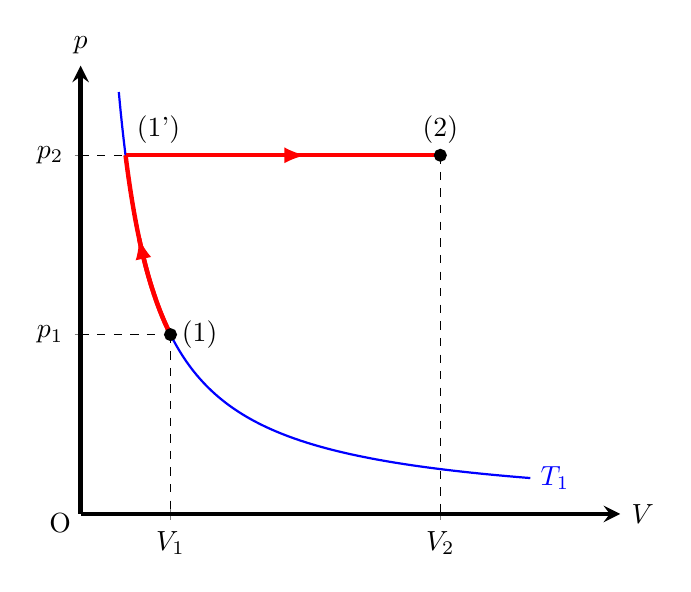
\begin{tikzpicture}  
					\begin{axis}[  ultra thick,
						xmin=0,  
						xmax=12,  
						ytick={3,6},
						xtick={2,8},
						ymin=0,  
						ymax=7.5, 
						samples=300,
						yticklabels={$p_1$, $p_2$},
						xticklabels={$V_1$, $V_2$},
						axis lines=center, 
						xlabel=$V$, 
						ylabel=$p$, 
						every axis y label/.style={at=(current axis.above origin),anchor=south},  
						every axis x label/.style={at=(current axis.right of origin),anchor=west},  ]
						\draw[line width=0.5pt, dashed] (axis cs: 0, 6) -- (axis cs: 8, 6);
						\draw[line width=0.5pt, dashed] (axis cs: 8, 6) -- (axis cs: 8, 0);
						\draw[line width=0.5pt, dashed] (axis cs: 0, 3) -- (axis cs: 2, 3);
						\draw[line width=0.5pt, dashed] (axis cs: 2, 3) -- (axis cs: 2, 0);
						\addplot [thick, blue, smooth, domain=0.85:10] {6/x} node[right] {$T_1$};  
						\addplot [ultra thick, red, smooth, domain=1:2] {6/x} ; 
						\addplot [ultra thick,-latex, red, smooth, domain=2:1.3] {6/x} ; 
						\addplot [ultra thick, red, smooth, domain=1:8] {6}; 
						\addplot [ultra thick,-latex, red, smooth, domain=1:5] {6};
						\filldraw[black] (axis cs:2,3) circle (1.5pt) node[right] {(1)};
						\filldraw[black] (axis cs:8,6) circle (1.5pt) node[above] {(2)};
						\node[above right] at (axis cs:1,6) {(1')};
					\end{axis}  
					\node[label={[below left]90:O}] at (0,0){};
				\end{tikzpicture}
				\captionof{figure}{Sơ đồ quá trình biến đổi trạng thái $(1)\rightarrow(1')\rightarrow(2)$}
			\end{center}
			\begin{enumerate}[label=\alph*)]
				\item Chứng minh rằng $\dfrac{p_1V_1}{T_1}=\dfrac{p_2V_2}{T_2}$. Từ đó suy ra $\dfrac{pV}{T}=C$ với $C$ là hằng số phụ thuộc vào số mol khí.
				\item Xác định giá trị của $C$ theo số mol $ n$.
			\end{enumerate}
	\loigiai{
				\begin{enumerate}[label=\alph*)]
					\item Xét quá trình biến đổi trạng thái của khối khí trong từng giai đoạn:\\
					\textbf{* Quá trình biến đổi trạng thái $(1)\rightarrow(1')$:}
					\begin{center}
						\begin{tabular}{C{4cm} C{1.5cm} C{5cm}}
							\colorbox{yellow}{\textcolor{red}{\textbf{Trạng thái 1}}} & $\xrightarrow[]{T=const}$ & \colorbox{yellow}{\textcolor{red}{\textbf{Trạng thái 1'}}}\\
							$V_1$ & &$V_1'$\\
							$p_1$ & & $p_1'=p_2$
						\end{tabular}
					\end{center}
					Theo định luật Boyle:
					\begin{equation}
						\label{eq:12.1}
						p_1V_1=p_1'V_1'\Leftrightarrow p_1V_1=p_2V_1'
					\end{equation}
					\textbf{* Quá trình biến đổi $(1')\rightarrow(2)$:}
					\begin{center}
						\begin{tabular}{C{4cm} C{1.5cm} C{5cm}}
							\colorbox{green!40!white}{\textcolor{red}{\textbf{Trạng thái 1'}}} & $\xrightarrow[]{p=const}$ & \colorbox{green!40!white}{\textcolor{red}{\textbf{Trạng thái 2}}}\\
							$V_1'$ & &$V_2$\\
							$T_1'=T_1$ & & $T_2$
						\end{tabular}
					\end{center}
					Theo định luật Charles:
					\begin{equation}
						\label{eq:12.2}
						\dfrac{V_1'}{T_1'}=\dfrac{V_2}{T_2}\Rightarrow V_1'=\dfrac{V_2T_1}{T_2}
					\end{equation}
					Thay phương trình (\ref{eq:12.1}) vào phương trình (\ref{eq:12.2}):
					$$p_1V_1=\dfrac{p_2V_2T_1}{T_2}\Rightarrow \dfrac{p_1V_1}{T_1}=\dfrac{p_2V_2}{T_2}$$
					hay
					\begin{equation}
						\label{eq:12.3}
						\dfrac{pV}{T}=C\quad(\text{đpcm}).
					\end{equation}
					\item Xét trong điều kiện tiêu chuẩn $p=\SI{1}{atm}=\SI{1.013E5}{\pascal}$; nhiệt độ $T=\SI{273}{\kelvin}$ và thể tích của $\xsi{ n}{\left(\mole\right)}$ khí $V=\xsi{22,4 n}{\left(\text{lít}\right)}=\xsi{0,0224 n}{\meter^3}$.\\
					Thay vào (\ref{eq:12.3}):
					$$C=\dfrac{pV}{T}=\dfrac{\left(\SI{1.013E5}{\pascal}\right)\cdot\left(\SI{0.0224}{\meter^3}\right)\cdot n}{\SI{273}{\kelvin}}\approx\xsi{8,31 n}{\left(\dfrac{\joule}{\mole\cdot\kelvin}\right)}.$$
				\end{enumerate}
		}
\end{vd}

\begin{dang}{Vận dụng được phương trình trạng thái của khí lí tưởng}
\end{dang}
\begin{vd}
	Trong cylanh của một động cơ đốt trong có $\SI{0.5}{\text{lít}}$ hỗn hợp khí ở áp suất $\SI{1}{atm}$ và nhiệt độ $\SI{47}{\celsius}$. Ấn piston xuống làm cho thể tích của hỗn hợp khí chỉ còn $\SI{0.05}{\text{lít}}$ và áp suất tăng lên $\SI{15}{atm}$. Giả thiết rằng hỗn hợp khí tăng tuân theo phương trình trạng thái của khí lí tưởng. Tính nhiệt độ của hỗn hợp khí ở trạng thái nén.
\loigiai{
	\begin{center}
		\begin{tabular}{C{4cm} C{1.5cm} C{5cm}}
			\colorbox{green!40!white}{\textcolor{red}{\textbf{Trạng thái đầu}}} & $\xrightarrow[]{ n=const}$ & \colorbox{green!40!white}{\textcolor{red}{\textbf{Trạng thái sau}}}\\
			$p_1=\SI{1}{atm}$ & & $p_2=\SI{15}{atm}$\\
			$V_1=\SI{0.5}{\text{lít}}$ & &$V_2=\SI{0.05}{\text{lít}}$\\
			$T_1=\SI{320}{\kelvin}$ & & $T_2=?$
		\end{tabular}
	\end{center}
	Do lượng khí là không đổi, áp dụng phương trình trạng thái của khí lí tưởng:
	$$\dfrac{p_1V_1}{T_1}=\dfrac{p_2V_2}{T_2}$$
	$$\Rightarrow T_2=\dfrac{p_2V_2}{p_1V_1}\cdot T_1=\dfrac{\left(\SI{15}{atm}\right)\cdot\left(\SI{0.05}{\text{lít}}\right)}{\left(\SI{1}{atm}\right)\cdot\left(\SI{0.5}{\text{lít}}\right)}\cdot\left(\SI{320}{\kelvin}\right)=\SI{480}{\kelvin}.$$
}
\end{vd}
% =================================================================		
\begin{vd}
	Tăng đồng thời nhiệt độ của một khối khí lí tưởng từ $\SI{27}{\celsius}$ lên $\SI{177}{\celsius}$ và áp suất từ $\SI{100}{\kilo\pascal}$ lên $\SI{300}{\kilo\pascal}$. Hỏi khối lượng riêng của khối khí tăng hay giảm bao nhiêu lần?
\loigiai{
		\begin{center}
			\begin{tabular}{C{4cm} C{1.5cm} C{5cm}}
				\colorbox{green!40!white}{\textcolor{red}{\textbf{Trạng thái đầu}}} & $\xrightarrow[]{ n=const}$ & \colorbox{green!40!white}{\textcolor{red}{\textbf{Trạng thái sau}}}\\
				$p_1=\SI{100}{\kilo\pascal}$ & & $p_2=\SI{300}{\kilo\pascal}$\\
				$T_1=\SI{300}{\kelvin}$ & & $T_2=\SI{450}{\kelvin}$\\
				$\rho_1, V_1$ & & $\rho_2, V_2$
			\end{tabular}
		\end{center}
		Gọi $\rho_1$, $V_1$ và $\rho_2$, $V_2$ lần lượt là khối lượng riêng, thể tích lúc đầu và lúc sau của khối khí đang xét; $m$ là khối lượng của khối khí.\\
		Áp dụng phương trình trạng thái của khí lí tưởng:
		$$pV=\dfrac{m}{\mu}RT\Rightarrow \rho=\dfrac{m}{V}=\dfrac{p\mu}{RT}.$$
		Như vậy:
		$$\dfrac{\rho_2}{\rho_1}=\dfrac{p_2}{p_1}\cdot\dfrac{T_1}{T_2}=\dfrac{\SI{300}{\kilo\pascal}}{\SI{100}{\kilo\pascal}}\cdot\dfrac{\SI{300}{\kelvin}}{\SI{450}{\kelvin}}=2.$$
		Như vậy, khối lượng riêng của khối khí lí tưởng này tăng 2 lần.
}
\end{vd}
	
% =============================================================
\begin{vd}
	\immini{
	Một cylanh đặt thẳng đứng có tiết diện là $S=\SI{100}{\centi\meter^2}$, chứa không khí ở nhiệt độ $t_1=\SI{27}{\celsius}$. Ban đầu cylanh được đậy bằng một piston cách đáy $h=\SI{50}{\centi\meter}$. Piston có thể trượt không ma sát dọc theo mặt trong cylanh. Đặt lên trên piston một quả cân có trọng lượng $P=\SI{500}{\newton}$. Piston dịch chuyển xuống đoạn $\ell=\SI{10}{\centi\meter}$ rồi dừng lại.\\
	Tính nhiệt độ của khí trong cylanh sau khi piston dừng lại. Biết áp suất khí quyển là $p_0=\SI{E5}{\newton/\meter^2}$. Bỏ qua khối lượng của piston.
}
{
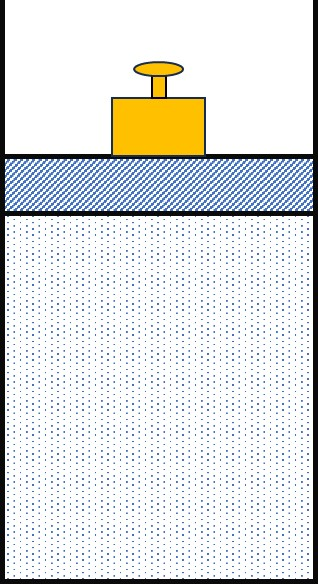
\includegraphics[scale=0.35]{figs/VN12-Y24-PH-SYL-012-1}
}
\loigiai{
	Ban đầu khi piston cân bằng, áp lực do khí quyển tác dụng lên piston bằng áp lực do khí trong bình tác dụng:
	$$p_1=p_0=\SI{E5}{\pascal}.$$
	Khi đặt quả cân lên piston và piston lại cân bằng, áp lực của khí trong cylanh tác dụng lên piston bằng áp lực khí quyển và trọng lực của quả cân:
	$$p_2=p_0+\dfrac{P}{S}=\SI{E5}{\pascal}+\dfrac{\SI{500}{\newton}}{\SI{100E-4}{\meter^2}}=\SI{1.5E5}{\pascal}.$$
	\begin{center}
		\begin{tabular}{C{4cm} C{1.5cm} C{5cm}}
			\colorbox{green!40!white}{\textcolor{red}{\textbf{Trạng thái đầu}}} & $\xrightarrow[]{ n=const}$ & \colorbox{green!40!white}{\textcolor{red}{\textbf{Trạng thái sau}}}\\
			$p_1=\SI{E5}{\pascal}$ & & $p_2=\SI{1.5E5}{\pascal}$\\
			$V_1=Sh$ & & $V_2=S\left(h-\ell\right)$\\
			$T_1=\SI{300}{\kelvin}$ & & $T_2=?$
		\end{tabular}
	\end{center}
	Áp dụng phương trình trạng thái của khí lí tưởng:
	$$\dfrac{p_1V_1}{T_1}=\dfrac{p_2V_2}{T_2}$$
	$$\Rightarrow T_2=\dfrac{p_2}{p_1}\cdot\dfrac{V_2}{V_1}\cdot T_1=\dfrac{p_2}{p_1}\cdot\dfrac{\left(h-\ell\right)}{h}\cdot T_1$$
	$$\Leftrightarrow T_2=\dfrac{\SI{1.5E5}{\pascal}}{\SI{E5}{\pascal}}\cdot\left(\dfrac{\SI{50}{\centi\meter}-\SI{10}{\centi\meter}}{\SI{50}{\centi\meter}}\right)\cdot\left(\SI{300}{\kelvin}\right)=\SI{360}{\kelvin}.$$
}
\end{vd}

\begin{dang}{Vận dụng được định luật Dalton \textit{(mở rộng)}}
Ở một nhiệt độ và thể tích xác định, áp suất toàn phần của một hỗn hợp khí gồm các khí không phản ứng hoá học với nhau bằng tổng áp suất riêng phần của mỗi khí thành phần có trong hỗn hợp:
		\begin{equation}
			p=p_1+p_2+\dots+p_n=\sum_{1}^{n}p_i
	\end{equation}
\end{dang}
\begin{vd}
	Bình A có dung tích $V_1=\SI{3}{\text{lít}}$, chứa một chất khí ở áp suất $p_1=\SI{2}{at}$. Bình B dung tích $V_2=\SI{4}{\text{lít}}$, chứa một chất khí ở áp suất $p_2=\SI{1}{at}$. Nhiệt độ trong hai bình là như nhau. Nối hai bình A, B thông với nhau bằng một ống dẫn nhỏ. Biết không có phản ứng hoá học xảy ra giữa hai khí trong các bình. Tính áp suất của hỗn hợp khí.
	\loigiai{Gọi áp suất riêng phần của mỗi khí trong hỗn hợp khi hai bình thông với nhau là $p_1'$ và $p_2'$.\\
			Trong quá trình nối hai bình với nhau, nhiệt độ của khí trong hai bình không đổi.\\
			\textbf{* Xét quá trình biến đổi trạng thái của khí trong bình A}
			\begin{center}
				\begin{tabular}{C{4cm} C{1.5cm} C{5cm}}
					\colorbox{yellow}{\textcolor{red}{\textbf{Trạng thái 1}}} & $\xrightarrow[]{T=const}$ & \colorbox{yellow}{\textcolor{red}{\textbf{Trạng thái 1'}}}\\
					$V_1=\SI{3}{\text{lít}}$ & &$V_1'=V_1+V_2=\SI{7}{\text{lít}}$\\
					$p_1=\SI{2}{at}$ & & $p_1'=?$
				\end{tabular}
			\end{center}
			Theo định luật Boyle:
			$$p_1V_1=p_1'V_1'\Rightarrow p_1'=\dfrac{p_1V_1}{V_1'}=\dfrac{\left(\SI{2}{at}\right)\cdot\left(\SI{3}{\text{lít}}\right)}{\SI{7}{\text{lít}}}=\xsi{\dfrac{6}{7}}{at}.$$
			\textbf{* Xét quá trình biến đổi trạng thái của khí trong bình B}
			\begin{center}
				\begin{tabular}{C{4cm} C{1.5cm} C{5cm}}
					\colorbox{green!40!white}{\textcolor{red}{\textbf{Trạng thái 2}}} & $\xrightarrow[]{T=const}$ & \colorbox{green!40!white}{\textcolor{red}{\textbf{Trạng thái 2'}}}\\
					$V_2=\SI{4}{\text{lít}}$ & &$V_2'=V_1+V_2=\SI{7}{\text{lít}}$\\
					$p_2=\SI{1}{at}$ & & $p_2'=?$
				\end{tabular}
			\end{center}
			Theo định luật Boyle:
			$$p_2V_2=p_2'V_2'\Rightarrow p_2'=\dfrac{p_2V_2}{V_2'}=\dfrac{\left(\SI{1}{at}\right)\cdot\left(\SI{4}{\text{lít}}\right)}{\SI{7}{\text{lít}}}=\xsi{\dfrac{4}{7}}{at}.$$
			Áp dụng định luật Dalton, áp suất của hỗn hợp khí:
			$$p'=p_1'+p_2'=\xsi{\dfrac{10}{7}}{at}\approx\SI{1.43}{at}.$$
	}
\end{vd}
\subsection{BÀI TẬP TRẮC NGHIỆM}
\setcounter{ex}{0}
\Opensolutionfile{ans}[ans/G12Y24B11TN]
% ===================================================================
\begin{ex}
	Một bình cầu thủy tinh chứa (không đầy) một lượng nước nóng có nhiệt độ khoảng $\SI{80}{\celsius}$ và được nút kín. Dội nước lạnh lên phần trên gần cổ bình, ta thấy nước trong bình lại sôi là vì
	\begin{enumerate}[label=(\arabic*)]
		\item Nhiệt độ sôi của chất lỏng phụ thuộc áp suất chất khí ở phía trên bề mặt chất lỏng: Áp suất giảm - nhiệt độ sôi giảm.
		\item Khi dội nước lạnh lên phần trên gần cổ bình sẽ làm cho nhiệt độ hơi bên trong giảm, kéo
		theo áp suất khí trên bề mặt chất lỏng giảm và do đó nhiệt độ sôi giảm xuống đến $\SI{80}{\celsius}$ nên ta thấy nước trong bình lại sôi.
	\end{enumerate}
	Giải thích đúng là
	
	\choice
	{chỉ (1)}
	{chỉ (2)}
	{\True (1) và (2)}
	{(1) và (2) đều sai}
	\loigiai{}
\end{ex}
% ===================================================================
\begin{ex}
	Biểu diễn hai đường đẳng tích của một khối khí lí tưởng trong hệ toạ độ $OpT$. Biểu thức so sánh $V_1$ và $V_2$ đúng là
	\begin{center}
		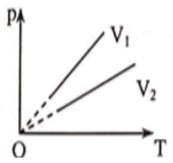
\includegraphics[width=0.2\linewidth]{figs/VN12-Y24-PH-SYL-012P-1}
	\end{center}
	\choice
	{$V_1>V_2$}
	{\True $V_1<V_2$}
	{$V_1=V_2$}
	{$V_1\ge V_2$}
	\loigiai{}
\end{ex}
% ===================================================================
\begin{ex}
Trên đồ thị $OVT$ vẽ bốn đường đẳng áp của cùng một lượng khí. Đường ứng với áp suất cao nhất là
\begin{center}
	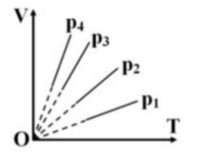
\includegraphics[width=0.2\linewidth]{figs/VN12-Y24-PH-SYL-012P-2}
\end{center}
	\choice
	{\True $p_1$}
	{$p_2$}
	{$p_3$}
	{$p_4$}
	\loigiai{}
\end{ex}
% ===================================================================
\begin{ex}
	Khi nitrogen được thu trên mặt nước ở nhiệt độ $\SI{25}{\celsius}$. Nếu áp suất hơi của nước ở $\SI{25}{\celsius}$ là $\SI{23.8}{\milli\meter Hg}$ và áp suất tổng cộng của hỗn hợp khí (gọi là khí nitrogen ướt) trong bình đo được là $\SI{735}{\milli\meter Hg}$ thì áp suất riêng phần của khí nitrogen (khí khô) là
	\choice
	{$\SI{760}{\milli\meter Hg}$}
	{$\SI{785.8}{\milli\meter Hg}$}
	{$\SI{710.8}{\milli\meter Hg}$}
	{\True $\SI{711.2}{\milli\meter Hg}$}
	\loigiai{}
\end{ex}
% ===================================================================
\begin{ex}
	Nén $\SI{10}{\liter}$ khí ở nhiệt độ $\SI{27}{\celsius}$ để cho thể tích của nó chỉ còn $\SI{4}{\liter}$. Trong quá trình nén, nhiệt độ khí tăng $\SI{33}{\celsius}$. So với áp suất ban đầu, áp suất khí lúc sau
	
	\choice
	{\True tăng 2,775 lần}
	{giảm 2,775 lần}
	{giảm 2,55 lần}
	{tăng 2,55 lần}
	\loigiai{\begin{center}
			\begin{tabular}{C{4cm} C{3cm} C{4cm}}
				\colorbox{yellow}{\textcolor{red}{\textbf{Trạng thái 1}}} & $\xrightarrow[]{\nu=\text{const}}$ & \colorbox{yellow}{\textcolor{red}{\textbf{Trạng thái 2}}}\\
				$p_1$ & &$p_2=?p_1$\\
				$V_1=\SI{10}{\liter}$ & & $V_2=\SI{4}{\liter}$\\
				$T_1=\SI{300}{\kelvin}$ & & $T_2=\SI{333}{\kelvin}$
			\end{tabular}
		\end{center}
		$$\dfrac{p_1V_1}{T_1}=\dfrac{p_2V_2}{T_2}\Rightarrow \dfrac{p_2}{p_1}=\dfrac{V_1}{V_2}\cdot\dfrac{T_2}{T_1}=2,775.$$
	}
\end{ex}
% ===================================================================
\begin{ex}
	Một bình cầu dung tích $\SI{20}{\liter}$ chứa khí oxygen ở nhiệt độ $\SI{16}{\celsius}$ và áp suất $\SI{100}{atm}$. Thể tích của lượng khí này ở điều kiện tiêu chuẩn là
	\choice
	{$\SI{34125}{\liter}$}
	{$\SI{2117}{\liter}$}
	{\True $\SI{1889}{\liter}$}
	{$\SI{125}{\liter}$}
	\loigiai{\begin{center}
			\begin{tabular}{C{4cm} C{3cm} C{4cm}}
				\colorbox{yellow}{\textcolor{red}{\textbf{Trạng thái 1}}} & $\xrightarrow[]{\nu=\text{const}}$ & \colorbox{yellow}{\textcolor{red}{\textbf{Trạng thái 2}}}\\
				$p_1=\SI{100}{atm}$ & &$p_2=\SI{1}{atm}$\\
				$V_1=\SI{20}{\liter}$ & & $V_2=?$\\
				$T_1=\SI{289}{\kelvin}$ & & $T_2=\SI{273}{\kelvin}$
			\end{tabular}
		\end{center}
		$$\dfrac{p_1V_1}{T_1}=\dfrac{p_2V_2}{T_2}\Rightarrow V_2\approx\SI{1889}{\liter}.$$}
\end{ex}
% ===================================================================
\begin{ex}
	Piston của một máy nén, sau mỗi lần nén đưa được $\SI{4}{\liter}$ khí ở nhiệt độ $\SI{27}{\celsius}$ và áp suất $\SI{1}{atm}$ vào bình chứa khí ở thể tích $\SI{2}{\meter^3}$. Nhiệt độ trong bình là $\SI{42}{\celsius}$. Áp suất khí trong bình khi piston đã thực hiện 1000 lần nén là
	
	\choice
	{\True $\SI{2.1}{atm}$}
	{$\SI{1.9}{atm}$}
	{$\SI{3.1}{atm}$}
	{$\SI{4.8}{atm}$}
	\loigiai{\begin{center}
			\begin{tabular}{C{4cm} C{3cm} C{4cm}}
				\colorbox{yellow}{\textcolor{red}{\textbf{Trạng thái 1}}} & $\xrightarrow[]{\nu=\text{const}}$ & \colorbox{yellow}{\textcolor{red}{\textbf{Trạng thái 2}}}\\
				$p_1=\SI{1}{atm}$ & &$p_2=\SI{0}{atm}$\\
				$V_1=\SI{4000}{\liter}$ & & $V_2=\SI{2000}{\liter}$\\
				$T_1=\SI{300}{\kelvin}$ & & $T_2=\SI{315}{\kelvin}$
			\end{tabular}
		\end{center}
		$$\dfrac{p_1V_1}{T_1}=\dfrac{p_2V_2}{T_2}\Rightarrow
		p_2=\SI{2.1}{atm}.$$
	}
\end{ex}
% ===================================================================
\begin{ex}
	Trong một động cơ diesel, khối khí có nhiệt độ ban đầu là $\SI{627}{\celsius}$ được nén để thể tích giảm bằng $\dfrac{1}{3}$ thể tích ban đầu và áp suất tăng $\SI{20}{\percent}$ so với áp suất ban đầu. Nhiệt độ của khối khí sau khi nén bằng
	
	\choice
	{$\SI{360}{\celsius}$}
	{\True $\SI{87}{\celsius}$}
	{$\SI{267}{\celsius}$}
	{$\SI{251}{\celsius}$}
	\loigiai{\begin{center}
			\begin{tabular}{C{4cm} C{3cm} C{4cm}}
				\colorbox{yellow}{\textcolor{red}{\textbf{Trạng thái 1}}} & $\xrightarrow[]{\nu=\text{const}}$ & \colorbox{yellow}{\textcolor{red}{\textbf{Trạng thái 2}}}\\
				$p_1$ & &$p_2=1,2p_1$\\
				$V_1$ & & $V_2=\dfrac{V_1}{3}$\\
				$T_1=\SI{900}{\kelvin}$ & & $T_2=?$
			\end{tabular}
		\end{center}
		$$\dfrac{p_1V_1}{T_1}=\dfrac{p_2V_2}{T_2}\Rightarrow T_2=\SI{360}{\kelvin}\Rightarrow t_2=\SI{87}{\celsius}.$$
	}
\end{ex}
% ===================================================================
\begin{ex}
	Một khối khí lí tưởng xác định, khi nhiệt độ của khối khí tăng thêm $\SI{16}{\celsius}$ thì thể tích của nó giảm đi $\SI{10}{\percent}$ so với thể tích ban đầu, áp suất tăng thêm $\SI{20}{\percent}$ so với áp suất ban đầu. Nhiệt độ ban đầu của khối khí là
	
	\choice
	{$\SI{300}{\kelvin}$}
	{$\SI{216}{\kelvin}$}
	{\True $\SI{200}{\kelvin}$}
	{$\SI{289}{\kelvin}$}
	\loigiai{\begin{center}
			\begin{tabular}{C{4cm} C{3cm} C{4cm}}
				\colorbox{yellow}{\textcolor{red}{\textbf{Trạng thái 1}}} & $\xrightarrow[]{\nu=\text{const}}$ & \colorbox{yellow}{\textcolor{red}{\textbf{Trạng thái 2}}}\\
				$p_1$ & &$p_2=1,2p_1$\\
				$V_1$ & & $V_2=0,9V_1$\\
				$T_1$ & & $T_2=T_1+16$
			\end{tabular}
		\end{center}
		$$\dfrac{p_1V_1}{T_1}=\dfrac{p_2V_2}{T_2}\Rightarrow \dfrac{p_1V_1}{T_1}=\dfrac{1,2p_1\cdot0,9V_1}{T_1+16}\Rightarrow T_1=\SI{200}{\kelvin}.$$
	}
\end{ex}
% ===================================================================
\begin{ex}
	Một bóng thám không được chế tạo để có thể tăng bán kính lên tới $\SI{10}{\meter}$ khi bay ở tầng khí quyển có áp suất $\SI{0.03}{atm}$ và nhiệt độ $\SI{200}{\kelvin}$. Ban đầu, bóng được bơm khí ở áp suất $\SI{1}{atm}$ và nhiệt độ $\SI{300}{\kelvin}$. Bán kính của bóng sau khi bơm là
	
	\choice
	{$\SI{3.75}{\meter}$}
	{$\SI{3.45}{\meter}$}
	{$\SI{4.75}{\meter}$}
	{\True $\SI{3.56}{\meter}$}
	\loigiai{\begin{center}
			\begin{tabular}{C{4cm} C{3cm} C{4cm}}
				\colorbox{yellow}{\textcolor{red}{\textbf{Trạng thái 1}}} & $\xrightarrow[]{\nu=\text{const}}$ & \colorbox{yellow}{\textcolor{red}{\textbf{Trạng thái 2}}}\\
				$p_1=\SI{1}{atm}$ & &$p_2=\SI{0.03}{atm}$\\
				$V_1=\dfrac{4}{3}\pi r^3_1$ & & $V_2=\dfrac{4}{3}\pi r^3_2$\\
				$T_1=\SI{300}{\kelvin}$ & & $T_2=\SI{200}{\kelvin}$
			\end{tabular}
		\end{center}
		$$\dfrac{p_1V_1}{T_1}=\dfrac{p_2V_2}{T_2}\Rightarrow r_1\approx\SI{3.56}{\meter}.$$
	}
\end{ex}
% ===================================================================
\begin{ex}
Hai bình cầu được nối với nhau bằng một ống có khoá, chứa hai chất khí không tác dụng hoá học với nhau, ở cùng nhiệt độ. Áp suất khí trong hai bình là $p_1=\SI{2E5}{\newton/\meter^2}$ và $p_2=\SI{E6}{\newton/\meter^2}$. Mở khoá nhẹ nhàng để hai bình thông với nhau sao cho nhiệt độ không đổi. Khi cân bằng xảy ra, áp suất ở hai bình là $p=\SI{4E5}{\newton/\meter^2}$. Tỉ số thể tích của hai bình cầu $V_1/V_2$ là
	
	\choice
	{$5$}
	{\True $3$}
	{$\dfrac{1}{3}$}
	{$\dfrac{1}{5}$}
	\loigiai{Theo định luật Boyle:
		$$\begin{cases}
			p_1V_1=p'_1\left(V_1+V_2\right)\\
			p_2V_2=p'_2\left(V_1+V_2\right)
		\end{cases}\Rightarrow \begin{cases}
			p'_1=\dfrac{p_1V_1}{V_1+V_2}\\
			p'_2=\dfrac{p_2V_2}{V_1+V_2}
		\end{cases}$$
		Theo định luật Dalton:
		$$p'=p'_1+p'_2$$
		Đặt $V_1=kV_2$ ta thu được:
		$$p'=\dfrac{kp_1+p_2}{k+1}\Rightarrow k=3.$$
	}
\end{ex}
% ===================================================================
\begin{ex}
Một căn phòng có kích thước $\SI{8}{\meter}\times \SI{5}{\meter}\times\SI{4}{\meter}$. Ban đầu không khí trong phòng ở điều kiện tiêu chuẩn (nhiệt độ $\SI{0}{\celsius}$ và áp suất là $\SI{760}{\milli\meter Hg}$), sau đó nhiệt độ của không khí tăng lên tới $\SI{10}{\celsius}$ và áp suất $\SI{780}{\milli\meter Hg}$. Thể tích của lượng khí (ở nhiệt độ $\SI{10}{\celsius}$ và áp suất $\SI{780}{\milli\meter Hg}$) đã rời khỏi phòng \textbf{gần nhất} với giá trị nào sau đây?
	
	\choice
	{$\SI{1.59}{\meter^3}$}
	{$\SI{3.41}{\meter^3}$}
	{$\SI{2.82}{\meter^3}$}
	{\True $\SI{1.61}{\meter^3}$}
	\loigiai{\begin{center}
			\begin{tabular}{C{4cm} C{3cm} C{4cm}}
				\colorbox{yellow}{\textcolor{red}{\textbf{Trạng thái 1}}} & $\xrightarrow[]{\nu=\text{const}}$ & \colorbox{yellow}{\textcolor{red}{\textbf{Trạng thái 2}}}\\
				$p_1=\SI{760}{\milli\meter Hg}$ & &$p_2=\SI{780}{\milli\meter Hg}$\\
				$V_1=\SI{160}{\meter^3}$ & & $V_2=?$\\
				$T_1=\SI{273}{\kelvin}$ & & $T_2=\SI{283}{\kelvin}$
			\end{tabular}
		\end{center}
		$$\dfrac{p_1V_1}{T_1}=\dfrac{p_2V_2}{T_2}\Rightarrow V_2\approx\SI{161.61}{\meter^3}.$$
		$$\Rightarrow \Delta V=V_2-V_1=\SI{1.61}{\meter^3}.$$
	}
\end{ex}
% ===================================================================
\begin{ex}
Một cylanh có piston cách nhiệt và nằm ngang. Piston ở vị trí chia cylanh thành hai phần bằng nhau, chiều dài của mỗi phần là $\SI{30}{\centi\meter}$. Mỗi phần chứa một lượng khí như nhau ở nhiệt độ $\SI{17}{\celsius}$ và áp suất $\SI{2}{atm}$. Muốn piston di chuyển $\SI{2}{\centi\meter}$ thì phải đun nóng khí ở một phần lên thêm bao nhiêu độ? Áp suất khí khi piston đã dịch chuyển là bao nhiêu?
	
	\choice
	{$\SI{41.4}{\kelvin}$ và $\SI{1.875}{atm}$}
	{\True $\SI{41.4}{\kelvin}$ và $\SI{2.14}{atm}$}
	{$\SI{19.3}{\kelvin}$ và $\SI{2.14}{atm}$}
	{$\SI{19.3}{\kelvin}$ và $\SI{1.875}{atm}$}
	\loigiai{$$\dfrac{p_0V_0}{T_0}=\dfrac{p_1V_1}{T_1}=\dfrac{p_2V_2}{T_2}$$
		$$\Leftrightarrow \dfrac{\left(\SI{2}{atm}\right)\cdot\left(\SI{30}{\centi\meter}\right)}{\SI{290}{\kelvin}}=\dfrac{p\cdot\left(\SI{32}{\centi\meter}\right)}{T}=\dfrac{p\cdot\left(\SI{28}{\centi\meter}\right)}{\SI{290}{\kelvin}}\Rightarrow \begin{cases}
			p\approx\SI{2.14}{atm}\\
			T\approx\SI{331.4}{\kelvin}
		\end{cases}.$$
	}
\end{ex}
% ===================================================================
\begin{ex}
	Bình kín được ngăn làm hai phần bằng nhau bằng tấm cách nhiệt có thể dịch chuyển được. Biết mỗi bên có chiều dài $\SI{30}{\centi\meter}$ và nhiệt độ của khí trong bình là $\SI{27}{\celsius}$. Khi nung nóng 1 bên thêm $\SI{10}{\celsius}$ và làm lạnh phần còn lại đi $\SI{10}{\celsius}$ thì độ dịch chuyển của tấm cách nhiệt là
	\choice
	{\True $\SI{1}{\centi\meter}$}
	{$\SI{10}{\centi\meter}$}
	{$\SI{5}{\centi\meter}$}
	{$\SI{2}{\centi\meter}$}
	\loigiai{$$\dfrac{p_0V_0}{T_0}=\dfrac{p_1V_1}{T_1}=\dfrac{p_2V_2}{T_2}\Leftrightarrow \dfrac{p_0\cdot\left(\SI{30}{\centi\meter}\right)}{\SI{300}{\kelvin}}=\dfrac{p\cdot\left(30+x\right)}{\SI{310}{\kelvin}}=\dfrac{p\cdot\left(30-x\right)}{\SI{290}{\kelvin}}\Rightarrow x=\SI{1}{\centi\meter}.$$
	}
\end{ex}
% ===================================================================
\begin{ex}
Hai bình giống nhau được nối với nhau bằng một ống nằm ngang có tiết diện $\SI{20}{\milli\meter^2}$, giữa ống có một giọt thuỷ ngân. Ở $\SI{0}{\celsius}$, giọt thuỷ ngân ở chính giữa ống, thể tích khí ở mỗi ngăn là $V_0=\SI{200}{\centi\meter^3}$. Nếu nhiệt độ ở một bình là $\xsi{t}{\celsius}$ và bình kia là $\xsi{-t}{\celsius}$ thì giọt thuỷ ngân dịch chuyển $\SI{10}{\centi\meter}$. Giá trị của $t$ là	
	\choice
	{$\SI{13.65}{\celsius}$}
	{\True $\SI{2.73}{\celsius}$}
	{$\SI{27.3}{\celsius}$}
	{$\SI{1.365}{\celsius}$}
	\loigiai{$$\dfrac{p_0\cdot200}{273}=\dfrac{p\cdot202}{t+273}=\dfrac{p\cdot198}{-t+273}\Rightarrow t=\SI{2.73}{\celsius}.$$
	}
\end{ex}
% ===================================================================
\begin{ex}
Một cái hồ sâu $\SI{15}{\meter}$, dưới đáy hồ nhiệt độ của nước là $\SI{7}{\celsius}$ còn trên mặt hồ là $\SI{22}{\celsius}$. Một bọt không khí có thể tích $\SI{1}{\milli\meter^3}$ nổi lên từ đáy hồ. Biết áp suất khí quyển là $p_0=\SI{760}{\milli\meter Hg}$, khối lượng riêng của nước và của thuỷ ngân lần lượt là $\SI{1000}{\kilogram/\meter^3}$; $\SI{13600}{\kilogram/\meter^3}$. Ở sát mặt nước, thể tích bọt khí là	
	\choice
	{$\SI{1.5}{\milli\meter^3}$}
	{$\SI{3.3}{\milli\meter^3}$}
	{\True $\SI{2.6}{\milli\meter^3}$}
	{$\SI{2.7}{\milli\meter^3}$}
	\loigiai{\begin{center}
			\begin{tabular}{C{5cm} C{3cm} C{5cm}}
				\colorbox{yellow}{\textcolor{red}{\textbf{Trạng thái 1}}} & $\xrightarrow[]{\nu=\text{const}}$ & \colorbox{yellow}{\textcolor{red}{\textbf{Trạng thái 2}}}\\
				$p_1=p_0+\dfrac{h}{13,6}\approx\SI{1863}{\milli\meter Hg}$ & &$p_2=p_0=\SI{760}{\milli\meter Hg}$\\
				$V_1=\SI{1}{\milli\meter^3}$ & & $V_2=?$\\
				$T_1=\SI{280}{\kelvin}$ & & $T_2=\SI{295}{\kelvin}$
			\end{tabular}
		\end{center}
		$$\dfrac{p_1V_1}{T_1}=\dfrac{p_2V_2}{T_2}\Rightarrow V_2\approx\SI{2.6}{\milli\meter^3}.$$
	}
\end{ex}
% ===================================================================
\begin{ex}
	Một tàu ngầm lặn ở độ sâu $\SI{40}{\meter}$ trong nước. Người ta mở một bình chứa không khí dung tích $\SI{500}{\liter}$, áp suất $\SI{10}{\mega\pascal}$, nhiệt độ $\SI{27}{\celsius}$, để đẩy nước ra khỏi thùng chứa nước của tàu. Biết rằng sau khi mở thùng, nhiệt độ của không khí là $\SI{3}{\celsius}$. Lấy áp suất khí quyển $p_0=\SI{E5}{\pascal}$, khối lượng riêng của nước $\rho=\SI{1000}{\kilogram/\meter^3}$, gia tốc trọng trường $g=\SI{10}{\meter/\second^2}$. Thể tích nước bị đẩy ra là
	
	\choice
	{$\SI{27}{\meter^3}$}
	{\True $\SI{8.7}{\meter^3}$}
	{$\SI{2.7}{\meter^3}$}
	{$\SI{87}{\meter^3}$}
	\loigiai{\begin{center}
			\begin{tabular}{C{4cm} C{3cm} C{4cm}}
				\colorbox{yellow}{\textcolor{red}{\textbf{Trạng thái 1}}} & $\xrightarrow[]{\nu=\text{const}}$ & \colorbox{yellow}{\textcolor{red}{\textbf{Trạng thái 2}}}\\
				$p_1=\SI{10E6}{\pascal}$ & &$p_2=p_0+\rho gh=\SI{0.5E6}{\pascal}$\\
				$V_1=\SI{500}{\liter}$ & & $V_2=?$\\
				$T_1=\SI{300}{\kelvin}$ & & $T_2=\SI{276}{\kelvin}$
			\end{tabular}
		\end{center}
		$$\dfrac{p_1V_1}{T_1}=\dfrac{p_2V_2}{T_2}\Rightarrow V_2=\SI{9200}{\liter}.$$
		Thể tích nước bị đẩy ra:
		$$\Delta V=V_2-V_1=\SI{8700}{\liter}=\SI{8.7}{\meter^3}.$$}
\end{ex}
% ===================================================================
\begin{ex}
	Một ống nghiệm tiết diện đều có chiều dài $\SI{76}{\centi\meter}$, đặt thẳng đứng chứa một khối khí đến nửa ống, phía trên ống bị chặn bởi một cột thuỷ ngân. Nhiệt độ ban đầu của khối khí là $\SI{0}{\celsius}$. Áp suất khí quyển là $\SI{76}{\centi\meter Hg}$. Để một nửa cột thuỷ ngân bị trào ra ngoài thì phải đun nóng khối khí lên đến nhiệt độ
	\begin{center}
		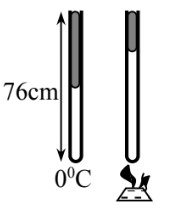
\includegraphics[width=0.15\linewidth]{figs/VN12-Y24-PH-SYL-012P-5}
	\end{center}
	
	\choice
	{$\SI{30}{\celsius}$}
	{$\SI{50}{\celsius}$}
	{\True $\SI{68}{\celsius}$}
	{$\SI{90}{\celsius}$}
	\loigiai{\begin{center}
			\begin{tabular}{C{4cm} C{3cm} C{4cm}}
				\colorbox{yellow}{\textcolor{red}{\textbf{Trạng thái 1}}} & $\xrightarrow[]{\nu=\text{const}}$ & \colorbox{yellow}{\textcolor{red}{\textbf{Trạng thái 2}}}\\
				$p_1=p_0+h_{\ce{Hg}}=\SI{114}{\centi\meter Hg}$ & &$p_2=p_0+\dfrac{h_{\ce{Hg}}}{2}=\SI{95}{\centi\meter Hg}$\\
				$V_1=\xsi{38S}{\centi\meter^3}$ & & $V_2=\xsi{57S}{\centi\meter^3}$\\
				$T_1=\SI{273}{\kelvin}$ & & $T_2=?$
			\end{tabular}
		\end{center}
		$$\dfrac{p_1V_1}{T_1}=\dfrac{p_2V_2}{T_2}\Rightarrow T_2\approx\SI{341}{\kelvin}\Rightarrow t_2=\SI{68}{\celsius}.$$
	}
\end{ex}
% ===================================================================
\begin{ex}
	Hai bình cầu cùng dung tích chứa một chất khí nối với nhau bằng ống ngang. Một giọt thuỷ ngân nằm chính giữa ống ngang. Nhiệt độ trong các bình tương ứng là $T_1$ và $T_2$. Tăng gấp đôi nhiệt độ tuyệt đối của khí trong mỗi bình thì giọt thuỷ ngân sẽ
	\begin{center}
		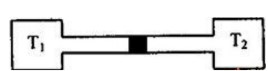
\includegraphics[width=0.35\linewidth]{figs/VN12-Y24-PH-SYL-012P-4}
	\end{center}
	
	\choice
	{\True nằm yên không chuyển động}
	{chuyển động sang phải}
	{chuyển động sang trái}
	{chưa đủ dữ kiện để xác định}
	\loigiai{$$\dfrac{pV}{T}=\text{const}\Rightarrow \begin{cases}
			\dfrac{pV}{T_1}=\dfrac{p'V_1}{2T_1}\\
			\dfrac{pV}{T_2}=\dfrac{p'V_2}{2T_2}
		\end{cases}\Rightarrow \begin{cases}
			pV=\dfrac{p'V_1}{2}\\
			pV=\dfrac{p'V_2}{2}
		\end{cases}\Rightarrow V_1=V_2.$$
		Vậy giọt thuỷ ngân không di chuyển}
\end{ex}
% ===================================================================
\begin{ex}
	Hai bình cầu cùng dung tích chứa một chất khí nối với nhau bằng ống ngang. Một giọt thuỷ ngân nằm chính giữa ống ngang. Nhiệt độ trong các bình tương ứng là $T_1$ và $T_2$. Tăng nhiệt độ khối khí trong mỗi bình thêm một lượng $\Delta T$ như nhau thì giọt thuỷ ngân sẽ 
	\begin{center}
		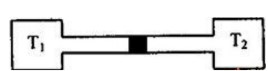
\includegraphics[width=0.35\linewidth]{figs/VN12-Y24-PH-SYL-012P-4}
	\end{center}
	
	\choice
	{nằm yên không chuyển động}
	{chuyển động sang phải}
	{chuyển động sang trái}
	{\True chưa đủ dữ kiện để xác định}
	\loigiai{$$\dfrac{pV}{T}=\text{const}\Rightarrow \begin{cases}
			\dfrac{pV}{T_1}=\dfrac{p'V_1}{T_1+\Delta T}\\
			\dfrac{pV}{T_2}=\dfrac{p'V_2}{T_2+\Delta T}
		\end{cases}\Rightarrow \begin{cases}
			V_1=\dfrac{pV}{p'}\left(1+\dfrac{\Delta T}{T_1}\right)\\
			V_2=\dfrac{pV}{p'}\left(1+\dfrac{\Delta T}{T_2}\right)\\
		\end{cases}.$$
		Vậy giọt thuỷ ngân di chuyển về phía nào còn phụ thuộc vào nhiệt độ ban đầu $T_1$, $T_2$ ở mỗi ngăn}
\end{ex}
\Closesolutionfile{ans}
\subsection{TRẮC NGHIỆM ĐÚNG/SAI}
\setcounter{ex}{0}
% ===================================================================
\begin{ex}
	Vào những ngày trời mát dịu, khi thổi bong bóng xà phòng, ta quan sát thấy lúc đầu bong bóng bay lên cao rồi dần dần rơi xuống (nếu bóng không vỡ giữa chừng). Nhận định các lời giải thích sau đây cho hiện tượng trên.
	\begin{center}
		
\includegraphics[width=0.2\linewidth]{figs/VN12-Y24-PH-SYL-011P-1}
	\end{center}
	\begin{enumerate}[label=\alph*)]
		\item Bong bóng xà phòng chủ yếu chịu tác dụng của trọng lực và lực nâng của không khí.
		\item Khi vừa được thổi, nhiệt độ không khí trong bong bóng cao hơn nhiệt độ môi trường, do đó lực nâng của không khí tác dụng lên bóng thắng được trọng lực của bóng làm bóng bay lên.
		\item Sau một thời gian, nhiệt độ của không khí trong bóng giảm để cân bằng với nhiệt độ môi trường.
		\item Trong quá trình nhiệt độ khí giảm, thể tích bong bóng tăng và làm giảm lực nâng của không khí lên bóng.
	\end{enumerate}
	
	\loigiai{\begin{enumerate}[label=\alph*)]
			\item Đúng.
			\item Đúng.
			\item Đúng.
			\item Sai. Nhiệt độ khí giảm thì thể tích khí trong bóng giảm.
	\end{enumerate}}
\end{ex}
% ===================================================================
\begin{ex}
	\immini{
Một lốp ô tô được bơm căng không khí ở nhiệt độ $\SI{27}{\celsius}$. Áp suất ban đầu của khí ở áp suất khí quyển bình thường là $\SI{1.013E5}{\pascal}$. Trong quá trình bơm, không khí vào trong lốp bị nén lại và giảm $\SI{80}{\percent}$ thể tích ban đầu (khi không khí còn ở bên ngoài lốp), nhiệt độ khí trong lốp tăng lên đến $\SI{40}{\celsius}$.	
\begin{enumerate}[label=\alph*)]
	\item Tỉ số thể tích sau khi đưa vào trong lốp và thể tích khí khi ở ngoài lốp là 0,2.
	\item Áp suất khí trong lốp là $\SI{2.11E3}{\pascal}$.
	\item Biết phần lốp xe tiếp xúc với mặt đường có diện tích $\SI{205}{\centi\meter^2}$. Áp lực của lốp xe tác dụng lên mặt đường cỡ $\SI{1000}{\newton}$.
	\item Sau khi ô tô chạy ở tốc độ cao, nhiệt độ không khí trong lốp tăng lên đến $\SI{75}{\celsius}$ và thể tích khí bên trong lốp tăng bằng $\SI{102}{\percent}$ thể tích lốp ở $\SI{40.0}{\celsius}$. Áp suất mới của khí trong lốp là $\SI{5.76E5}{\pascal}$.
	
\end{enumerate}

}
{
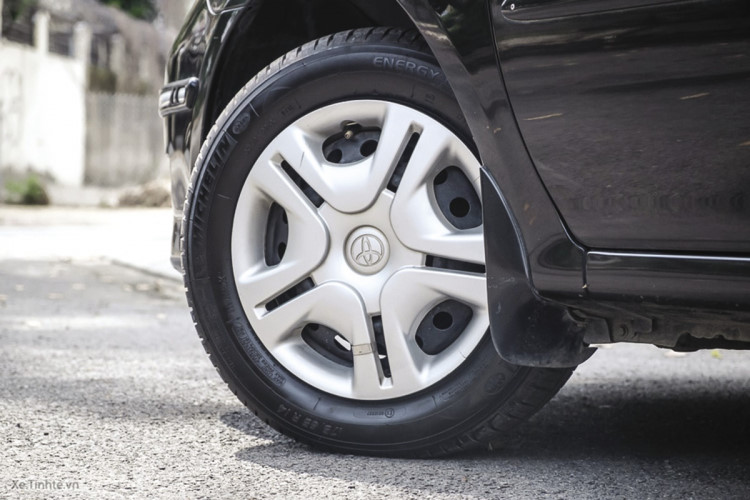
\includegraphics[scale=0.15]{figs/VN12-Y24-PH-SYL-012P-6}
}
	\loigiai{\begin{enumerate}[label=\alph*)]
			\item Đúng.
			\item Sai.
			$$\dfrac{p_1V_1}{T_1}=\dfrac{p_2V_2}{T_2}\Rightarrow p_2=p_1\cdot\dfrac{V_1}{V_2}\cdot\dfrac{T_2}{T_1}=\SI{5.28E5}{\pascal}.$$
			\item Sai. Áp dụng phương trình trạng thái:
			$$F=p_2S=\SI{10824}{\newton}.$$
			\item Đúng.\\
			$$p_3=p_2\cdot\dfrac{V_2}{V_3}\cdot\dfrac{T_3}{T_2}=\SI{5.76E5}{\pascal}.$$
			
		\end{enumerate}
	}
\end{ex}
% ===================================================================
\begin{ex}
\immini{
Một lọ giác hơi (được cơ sở điều trị bằng phương pháp cổ truyền sử dụng) do chênh lệch áp suất rong và ngoài lọ nên dính vào bề mặt da lưng của người bệnh, điều này được tạo ra bằng cách sau:\\
Ban đầu, người ta hơ nóng không khí bên trong lọ và nhanh chóng úp miệng hở của lọ vào vùng da cần tác động. Tại thời điểm áp vào da, nhiệt độ không khí trong lọ vào khoảng $t_1=\SI{353}{\celsius}$. Sau một thời gian, nhiệt độ không khí giảm dần và cân bằng nhiệt với không khí bên ngoài ở nhiệt độ khoảng $t_2=\SI{27}{\celsius}$. Áp suất khí quyển $p_0=\SI{E5}{\pascal}$. Diện tích phần miệng hở của lọ là $S=\SI{28.0}{\centi\meter^2}$. Bỏ qua sự thay đổi thể tích của không khí trong bình (do sự phồng lên của da bên trong miệng lọ).
}
{

\includegraphics[scale=0.5]{figs/VN12-Y24-PH-SYL-012P-8}
}
	\begin{enumerate}[label=\alph*)]
		\item Chênh lệch áp suất trong và ngaoij lọ giác hơi tạo lực hút làm máu dưới da tăng cường đến nơi miệng lọ giác hơi bám vào, từ đó tạo ra tác dụng lưu thông khí huyết.
		\item Áp suất khí trong lọ khi nhiệt độ khí cân bằng với nhiệt độ môi trường là $\SI{4.8E5}{\pascal}$.
		\item Lực hút tối đa lên mặt da là $\SI{156}{\newton}$.
		\item Thực tế, do bề mặt da bị phòng lên bên trong miệng của lọ nên thể tích khí trong lọ bị giảm $\SI{10}{\percent}$. Chênh lệch áp suất khí trong lọ và ngoài lọ là $\SI{5.3E4}{\pascal}$.
	\end{enumerate}
	
	\loigiai{\begin{enumerate}[label=\alph*)]
			\item Đúng.
			\item Đúng.
			\item Sai. $F=\left(p_0-p_2\right)S=\SI{145.6}{\newton}$.
			\item Sai. 
			$$\dfrac{p\cdot 0,9V_0}{T}=\dfrac{p_0V_0}{T_0}\Rightarrow p=\SI{5.3E4}{\pascal}.$$
			Chênh lệch áp suất trong và ngoài lọ:
			$$\Delta p=p_0-p=\SI{4.7E4}{\pascal}.$$
	\end{enumerate}}
\end{ex}
% ===================================================================
\begin{ex}
\immini{
Một khách du lịch đang đi dạo ở Đà Lạt, người này sau khi uống hết nước trong chai thể tích $\SI{500}{\milli\liter}$ thì đóng nắp chai nước lại và mang theo người, chai nước có vỏ rất mỏng. Nhiệt độ tại Đà Lạt vào thời điểm đó là $\SI{25}{\celsius}$.\\
Tại những nơi ở gần mặt đất và nhiệt độ thay đổi không đáng kể, áp suất khí quyển thay đổi theo độ cao $h$ so với mặt nước biển $p=p_0e^{-0,00011h}$, trong đó $p_0$ là áp suất khí quyển tại mặt đất ngang với mặt nước biển và bằng $\SI{1}{atm}$, $h$ có đơn vị mét. Thành phố Đà Lạt ở độ cao $\SI{1500}{\meter}$ so với mặt nước biển.
}	
{
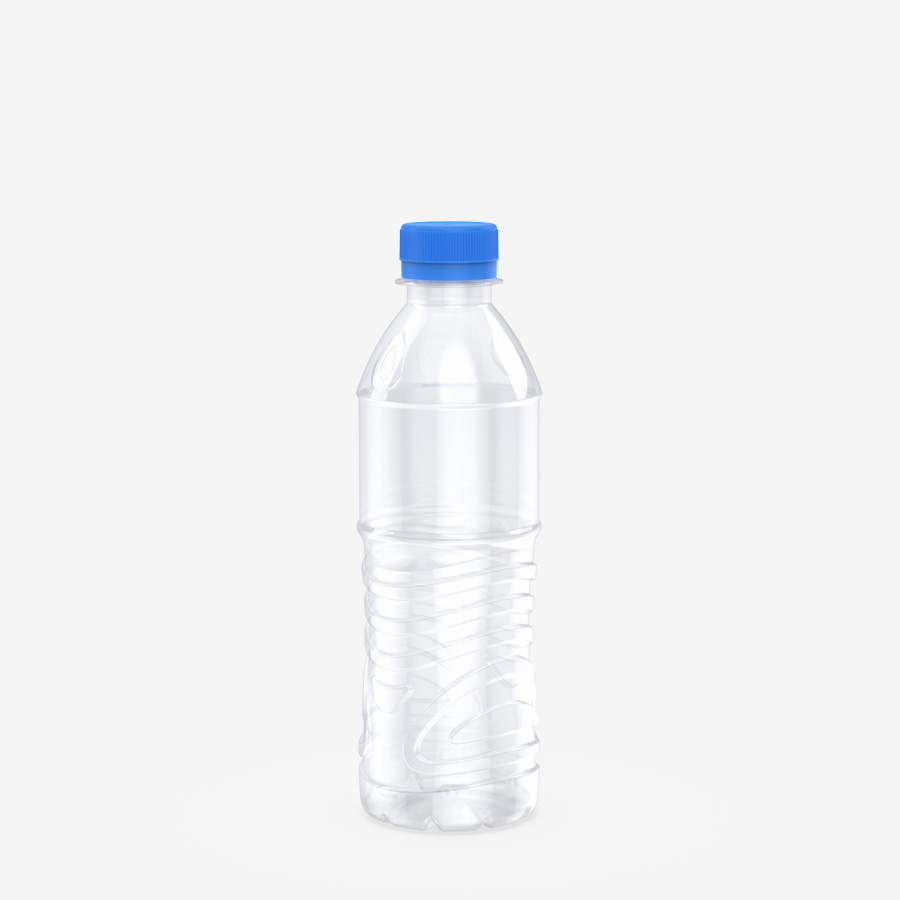
\includegraphics[scale=0.1]{figs/VN12-Y24-PH-SYL-012P-7}
}
\begin{enumerate}[label=\alph*)]
	\item Áp suất khí quyển tại Đà Lạt xấp xỉ $\SI{0.848}{atm}$.
	\item Khi mang chai nước lên xe khách đang mở điều hoà ở nhiệt độ $\SI{20}{\celsius}$ thì người này thấy vỏ chai bị phồng lên.
	\item Khi về đến Thành phố Hồ Chí Minh (có độ cao ngang mực nước biển và nhiệt độ $\SI{32}{\celsius})$, người này thấy chai nước bị dẹp đi.
	\item Chai nước sẽ trở lại hình dạng bình thường nếu ở độ cao khoảng $\SI{1289}{\meter}$ với nhiệt độ $\SI{32}{\celsius}$.
\end{enumerate}
	\loigiai{\begin{enumerate}[label=\alph*)]
			\item Đúng.
			\item Sai. Ở cùng điều kiện áp suất, nhiệt độ khí giảm thì thể tích khí giảm. Chai sẽ bị bẹp lại.
			\item Đúng.\\
			\begin{center}
				\begin{tabular}{C{4cm} C{3cm} C{4cm}}
					\colorbox{yellow}{\textcolor{red}{\textbf{Trạng thái ở Đà Lạt}}} & $\xrightarrow[]{\nu=\text{const}}$ & \colorbox{yellow}{\textcolor{red}{\textbf{Trạng thái ở Tp.HCM}}}\\
					$p_1=\SI{0.848}{atm}$ & &$p_2=?$\\
					$T_1=\SI{298}{\kelvin}$ & & $T_2=\SI{305}{\kelvin}$\\
					$V_1=\SI{500}{\liter}$ & & $V_2=?$\\
				\end{tabular}
			\end{center}
			Áp dụng phương trình trạng thái khí lí tưởng:
			$$\dfrac{p_1V_1}{T_1}=\dfrac{p_2V_2}{T_2}\Rightarrow V_2\approx\SI{434}{\milli\liter}.$$
			\item  Đúng.\\
			\begin{center}
				\begin{tabular}{C{4cm} C{3cm} C{4cm}}
					\colorbox{yellow}{\textcolor{red}{\textbf{Trạng thái ở Đà Lạt}}} & $\xrightarrow[]{V=\text{const}}$ & \colorbox{yellow}{\textcolor{red}{\textbf{Trạng thái ở độ cao $h$}}}\\
					$p_1=\xsi{e^{-0,00011\cdot1500}}{atm}$ & &$p_2=\xsi{e^{-0,00011\cdot h}}{atm}$\\
					$T_1=\SI{298}{\kelvin}$ & & $T_2=\SI{305}{\kelvin}$
				\end{tabular}
			\end{center}
			
			$$\dfrac{p_2}{p_1}=\dfrac{T_2}{T_1}\Rightarrow h\approx\SI{1289}{\meter}.$$
		\end{enumerate}
	}
\end{ex}
\subsection{BÀI TẬP TỰ LUẬN}
\setcounter{ex}{0}
% ===================================================================
\begin{ex}
	Trong cylanh của một động cơ đốt trong có $\SI{2}{\liter}$ hỗn hợp khí dưới áp suất $\SI{1.5}{atm}$ và nhiệt độ $\SI{47}{\celsius}$. Piston nén xuống làm cho thể tích của hỗn hợp khí chỉ còn $\SI{0.2}{\liter}$ và áp suất tăng đến $\SI{21}{atm}$. Tính nhiệt độ của hỗn hợp khí nén.
	\loigiai{\begin{center}
			\begin{tabular}{C{4cm} C{3cm} C{4cm}}
				\colorbox{yellow}{\textcolor{red}{\textbf{Trạng thái 1}}} & $\xrightarrow[]{\nu=\text{const}}$ & \colorbox{yellow}{\textcolor{red}{\textbf{Trạng thái 2}}}\\
				$p_1=\SI{1.5}{atm}$ & &$p_2=\SI{21}{atm}$\\
				$V_1=\SI{2}{\liter}$ & & $V_2=\SI{0.2}{\liter}$\\
				$T_1=\SI{320}{\kelvin}$ & & $T_2=?$
			\end{tabular}
		\end{center}
		$$\dfrac{p_1V_1}{T_1}=\dfrac{p_2V_2}{T_2}\Rightarrow T_2=\SI{448}{\kelvin}\Rightarrow t_2=\SI{175}{\celsius}.$$}
\end{ex}
% ===================================================================
\begin{ex}
	Trong cylanh của một động cơ đốt trong có $\SI{2}{\liter}$ hỗn hợp khí dưới áp suất $\SI{1.5}{atm}$ và nhiệt độ $\SI{27}{\celsius}$. Piston nén xuống làm cho thể tích của hỗn hợp khí chỉ còn bằng $\SI{0.3}{\liter}$ và áp suất tăng lên tới $\SI{18}{atm}$. Tính nhiệt độ của hỗn hợp khí nén.
	\loigiai{\begin{center}
			\begin{tabular}{C{4cm} C{3cm} C{4cm}}
				\colorbox{yellow}{\textcolor{red}{\textbf{Trạng thái 1}}} & $\xrightarrow[]{\nu=\text{const}}$ & \colorbox{yellow}{\textcolor{red}{\textbf{Trạng thái 2}}}\\
				$p_1=\SI{1.5}{atm}$ & &$p_2=\SI{18}{atm}$\\
				$V_1=\SI{2}{\liter}$ & & $V_2=\SI{0.3}{\liter}$\\
				$T_1=\SI{300}{\kelvin}$ & & $T_2=?$
			\end{tabular}
		\end{center}
		$$\dfrac{p_1V_1}{T_1}=\dfrac{p_2V_2}{T_2}\Rightarrow T_2=\SI{540}{\kelvin}\Rightarrow t_2=\SI{267}{\celsius}.$$}
\end{ex}
% ===================================================================
\begin{ex}
	Trong một khu hội chợ, người ta bơm một quả bóng có thể tích $\SI{200}{\liter}$ ở nhiệt độ $\SI{27}{\celsius}$ trên mặt đất. Sau đó, bóng được thả bay lên độ cao mà ở đó áp suất khí quyển chỉ còn 0,8 lần áp suất khí quyển ở mặt đất và có nhiệt độ $\SI{17}{\celsius}$. Tính thể tích của quả bóng ở độ cao đó, bỏ qua áp suất phụ gây ra bởi vỏ quả bóng.
	\loigiai{\begin{center}
			\begin{tabular}{C{4cm} C{3cm} C{4cm}}
				\colorbox{yellow}{\textcolor{red}{\textbf{Trạng thái 1}}} & $\xrightarrow[]{\nu=\text{const}}$ & \colorbox{yellow}{\textcolor{red}{\textbf{Trạng thái 2}}}\\
				$p_1$ & &$p_2=0,8p_1$\\
				$T_1=\SI{300}{\kelvin}$ & & $T_2=\SI{290}{\kelvin}$\\
				$V_1=\SI{200}{\liter}$ & & $V_2=?$
			\end{tabular}
		\end{center}
		$$\dfrac{p_1V_1}{T_1}=\dfrac{p_2V_2}{T_2}\Rightarrow V_2=\SI{241.67}{\liter}.$$
	}
\end{ex}
% ===================================================================
\begin{ex}
	Một bình thép dung tích $\SI{50}{\liter}$ chứa khí hydrogen ở áp suất $\SI{5}{\mega\pascal}$ và nhiệt độ $\SI{37}{\celsius}$. Dùng bình này bơm được bao nhiêu quả bóng bay nếu mỗi quả có dung tích $\SI{10}{\liter}$, áp suất $\SI{1.05E5}{\pascal}$, nhiệt độ bóng bay là $\SI{12}{\celsius}$.
	
	\loigiai{\begin{center}
		\begin{tabular}{C{4cm} C{3cm} C{4cm}}
			\colorbox{yellow}{\textcolor{red}{\textbf{Trạng thái 1}}} & $\xrightarrow[]{\nu=\text{const}}$ & \colorbox{yellow}{\textcolor{red}{\textbf{Trạng thái 2}}}\\
			$p_1=\SI{5E6}{\pascal}$ & &$p_2=\SI{1.05E5}{\pascal}$\\
			$T_1=\SI{310}{\kelvin}$ & & $T_2=\SI{285}{\kelvin}$\\
			$V_1=\SI{50}{\liter}$ & & $V_2=\SI{50}{\liter}+n\cdot\SI{10}{\liter}$
		\end{tabular}
	\end{center}
	Áp dụng phương trình trạng thái khí lí tưởng:
	$$\dfrac{p_1V_1}{T_1}=\dfrac{p_2V_2}{T_2}\Rightarrow n\approx214.$$}
\end{ex}
% ===================================================================
\begin{ex}
	Một thùng có thể tích $\SI{40}{\liter}$ chứa $\SI{3.96}{\kilogram}$ khí $\ce{CO_2}$, biết rằng bình khí sẽ nổ khi áp suất vượt quá $\SI{60}{atm}$. Khối lượng riêng của chất khí ở điều kiện tiêu chuẩn là $\SI{1.98}{\kilogram/\meter^3}$. Người ta cần phải bảo quản bình khí ở nhiệt độ bao nhiêu?
	\loigiai{\begin{center}
			\begin{tabular}{C{4cm} C{3cm} C{4cm}}
				\colorbox{yellow}{\textcolor{red}{\textbf{Trạng thái 1}}} & $\xrightarrow[]{\nu=\text{const}}$ & \colorbox{yellow}{\textcolor{red}{\textbf{Trạng thái 2}}}\\
				$p_1=\SI{1}{atm}$ & &$p_2=\SI{60}{atm}$\\
				$V_1=\dfrac{m}{\rho}=\SI{2}{\meter^3}$ & & $V_2=\SI{0.04}{\meter^3}$\\
				$T_1=\SI{273}{\kelvin}$ & & $T_2=?$
			\end{tabular}
		\end{center}
		$$\dfrac{p_1V_1}{T_1}=\dfrac{p_2V_2}{T_2}\Rightarrow T_2=\SI{372.6}{\kelvin}\Rightarrow t_2=\SI{54.6}{\celsius}.$$
		Vậy cần phải bảo quản bình khí ở nhiệt độ dưới $\SI{54.6}{\celsius}$.}
\end{ex}
% ===================================================================
\begin{ex}
	Một bình hình trụ dung tích $\SI{8}{\text{lít}}$, đặt thẳng đứng, đậy kín bằng một nắp khối lượng $\SI{2}{\kilogram}$ và có đường kính $\SI{20}{\centi\meter}$. Trong bình chứa khí ở nhiệt độ $\SI{100}{\celsius}$ và áp suất bằng áp suất khí quyển $\SI{E5}{\pascal}$. Khi nhiệt độ trong bình giảm còn $\SI{20}{\celsius}$ thì
	\begin{enumerate}[label=\alph*)]
		\item áp suất khí trong bình bằng bao nhiêu?
		\item muốn mở nắp bình cần một lực bằng bao nhiêu?
	\end{enumerate}
	\loigiai{\begin{enumerate}[label=\alph*)]
			\item Khí trong bình có khối lượng và thể tích không đổi:
			\begin{center}
				\begin{tabular}{C{4cm} C{1.5cm} C{5cm}}
					\colorbox{green!40!white}{\textcolor{red}{\textbf{Trạng thái 1}}} & $\xrightarrow[]{V=const}$ & \colorbox{green!40!white}{\textcolor{red}{\textbf{Trạng thái 2}}}\\
					$T_1=\SI{373}{\kelvin}$ & & $T_2=\SI{293}{\kelvin}$\\
					$p_1=\SI{E5}{\pascal}$ & & $p_2=?$
				\end{tabular}
			\end{center}
			Quá trình biến đổi trạng thái của khí trong bình là đẳng tích:
			$$\dfrac{p_1}{T_1}=\dfrac{p_2}{T_2}\Rightarrow p_2=\dfrac{p_1T_2}{T_1}=\dfrac{\left(\SI{E5}{\pascal}\right)\cdot\left(\SI{373}{\kelvin}\right)}{\SI{293}{\kelvin}}\approx\SI{7.86E4}{\pascal}.$$
			\item Muốn mở được nắp bình cần tác dụng vào nắp một lực tối thiểu để cùng với áp lực bên trong bình thắng trọng lực của nắp và áp lực của không khí bên ngoài:
			$$F+p_2S=mg+p_1S\Rightarrow F=mg+\left(p_1-p_2\right)\cdot\dfrac{\pi d^2}{4}=\left(\SI{2}{\kilogram}\right)\cdot\left(\SI{10}{\meter/\second^2}\right)+\left(\SI{E5}{\pascal}-\SI{7.86E4}{\pascal}\right)\cdot\dfrac{\pi \cdot\left(\SI{0.2}{\meter}\right)^2}{4}\approx\SI{692}{\newton}.$$
	\end{enumerate}}
\end{ex}
% ===================================================================
\begin{ex}
\immini{
Một cylanh đặt thẳng đứng có tiết diện là $S=\SI{100}{\centi\meter^2}$, chứa không khí ở nhiệt độ $t_1=\SI{27}{\celsius}$. Ban đầu cylanh được đậy bằng một piston cách đáy $h=\SI{50}{\centi\meter}$. Piston có thể di chuyển không ma sát dọc theo mặt trong của cylanh. Đặt lên trên piston một quả cân có trọng lượng $P=\SI{500}{\newton}$. Piston dịch chuyển xuống đoạn $\ell=\SI{10}{\centi\meter}$ rồi dừng lại. Biết áp suất khí quyển là $p_0=\SI{E5}{\pascal}$. Bỏ qua khối lượng của piston. Nhiệt độ của khí trong cylanh sau khi piston dừng lại là bao nhiêu?
}	
{
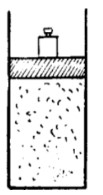
\includegraphics[scale=0.45]{figs/VN12-Y24-PH-SYL-012P-3}
}
	\loigiai{\begin{center}
			\begin{tabular}{C{4cm} C{3cm} C{4cm}}
				\colorbox{yellow}{\textcolor{red}{\textbf{Trạng thái 1}}} & $\xrightarrow[]{\nu=\text{const}}$ & \colorbox{yellow}{\textcolor{red}{\textbf{Trạng thái 2}}}\\
				$p_1=\SI{E5}{\pascal}$ & &$p_2=p_0+\dfrac{P}{S}=\SI{1.5E5}{\pascal}$\\
				$V_1=Sh=\SI{5000}{\centi\meter^3}$ & & $V_2=S\left(h-\ell\right)=\SI{4000}{\centi\meter^3}$\\
				$T_1=\SI{300}{\kelvin}$ & & $T_2=?$
			\end{tabular}
		\end{center}
		$$\dfrac{p_1V_1}{T_1}=\dfrac{p_2V_2}{T_2}\Rightarrow T_2=\SI{360}{\kelvin}\Rightarrow t_2=\SI{87}{\celsius}.$$
		
	}
\end{ex}
% ===================================================================
\begin{ex}
Cylanh kín được chia làm hai phần, mỗi phần dài $\SI{52}{\centi\meter}$ và ngăn cách nhau bằng piston cách nhiệt. Mỗi phần chứa một lượng khí giống nhau ở $\SI{27}{\celsius}$ và áp suất $\SI{75}{\centi\meter Hg}$. Khi nung nóng một phía của cylanh lên thêm $\SI{50}{\celsius}$ thì piston di chuyển. Áp suất khí trong cylanh sau khi nung là bao nhiêu?
	
	\loigiai{$$\dfrac{p_0V_0}{T_0}=\dfrac{p_1V_1}{T_1}=\dfrac{p_2V_2}{T_2}\Leftrightarrow\dfrac{\left(\SI{75}{\centi\meter Hg}\right)\cdot\left(\SI{52}{\centi\meter}\right)}{\SI{300}{\kelvin}}=\dfrac{p\cdot\left(52+x\right)}{\SI{350}{\kelvin}}=\dfrac{p\cdot\left(52-x\right)}{\SI{300}{\kelvin}}\Rightarrow\begin{cases}
			x=\SI{4}{\centi\meter}\\
			p=\SI{81.25}{\centi\meter Hg}
		\end{cases}.$$
	}
\end{ex}
% ===================================================================
\begin{ex}
Hai bình chứa cùng một lượng khí nối với nhau bằng một ống nằm ngang tiết diện $\SI{0.4}{\centi\meter^2}$, ngăn cách nhau bằng một giọt thuỷ ngân trong ống. Ban đầu mỗi phần có nhiệt độ $\SI{27}{\celsius}$ và thể tích $\SI{0.3}{\liter}$. Khi tăng nhiệt độ bình I thêm $\SI{2}{\celsius}$ và giảm nhiệt độ bình II đi $\SI{2}{\celsius}$ thì giọt thuỷ ngân di chuyển một khoảng bằng bao nhiêu và theo chiều nào?
	
	\loigiai{Gọi: \begin{itemize}
			\item $p_0$, $p$ lần lượt là áp suất mỗi bình ban đầu và sau khi thay đổi nhiệt độ;
			\item $x$ là khoảng dịch chuyển của giọt thuỷ ngân.
		\end{itemize}
		Áp dụng phương trình trạng khí lí tưởng cho mỗi bình trước và sau khi thay đổi nhiệt độ:
		$$\dfrac{p_0V_0}{T}=\dfrac{pV_1}{T_1}=\dfrac{pV_2}{T_2}$$
		$$\Leftrightarrow \dfrac{p\left(300+0,4x\right)}{302}=\dfrac{300-0,4x}{298}\Rightarrow x=\SI{5}{\centi\meter}.$$
	}
\end{ex}